\documentclass[a0,portrait,final]{a0poster}
% You might find the 'draft' option to a0 poster useful if you have
% lots of graphics, because they can take some time to process and
% display. (\documentclass[a0,draft]{a0poster})

% Switch off page numbers on a poster, obviously, and section numbers too.
\pagestyle{empty}
\setcounter{secnumdepth}{0}

% The textpos package is necessary to position textblocks at arbitary 
% places on the page.
\usepackage[absolute]{textpos}

% Graphics to include graphics. Times is nice on posters, but you
% might want to switch it off and go for CMR fonts.
\usepackage{graphics,wrapfig,times}

% These colours are tried and tested for titles and headers. Don't
% over use color!
\usepackage{color}
\definecolor{darkblue}{rgb}{0.1,0.1,0.5}
\definecolor{darkred}{rgb}{0.8,0.0,0.1}

% see documentation for a0poster class for the size options here
%\let\Textsize\normalsize
%\def\Head#1{\noindent\hbox to \hsize{\hfil{\LARGE\color{darkblue} #1}}\bigskip}
%\def\LHead#1{\noindent{\LARGE\color{darkblue} #1}\smallskip}
%\def\Subhead#1{\noindent{\large\color{darkblue} #1}}
%\def\Title#1{\noindent{\VeryHuge\color{darkred} #1}}

% Set up the grid
%
% Note that [40mm,40mm] is the margin round the edge of the page --
% it is _not_ the grid size. That is always defined as 
% PAGE_WIDTH/HGRID and PAGE_HEIGHT/VGRID. In this case we use
% 15 x 25. This gives us a wide central column for text (7 grid
% spacings) and two narrow columns (3 each) at each side for 
% pictures, separated by 1 grid spacing.
%
% Note however that texblocks can be positioned fractionally as well,
% so really any convenient grid size can be used.
%
\TPGrid[40mm,40mm]{15}{25}  % 3 - 1 - 7 - 1 - 3 Columns

% Mess with these as you like
\parindent=0pt
\parskip=0.8\baselineskip
\renewcommand{\baselinestretch}{0.95}


%\usepackage{amsmath,amsthm, amssymb, latexsym}
\usepackage{fix-cm}
\usepackage[english]{babel}
\usepackage[latin1]{inputenc}
\usepackage{times}
\usepackage[T1]{fontenc}
\usepackage{calc} 

% PGF includes
\usepackage{pgf}
\usepackage{tikz}
\usetikzlibrary{shadows,calc,plotmarks}
\usetikzlibrary{shapes,arrows}
\pgfdeclarelayer{background}
\pgfdeclarelayer{foreground}
\pgfsetlayers{background,main,foreground}
%\usetikzlibrary{,decorations,backgrounds,matrix,automata,trees,shapes,}


%\title[Learning BDI Plan Selection]{Learning Context Conditions for BDI Plan Selection}
%\author[Singh et al.]{Dhirendra~Singh\inst{1}, Sebastian~Sardina\inst{1}, Lin~Padgham\inst{1}, and St\'ephane~Airiau\inst{2}}

%\institute[RMIT \& UvA]{
%\inst{1}School of Computer Science \& Information Technology, RMIT University, Australia \\
%\inst{2}Institute for Logic, Language and Computation, University of Amsterdam, The Netherlands
%}

%\date[AAMAS 2010]{Autonomous Agents and Multiagent Systems\\May 2010}

\newcommand{\posterheading}[1]{
	\begin{center}
	  \begin{tikzpicture}
		\definecolor{darkblue}{rgb}{0.1,0.1,0.5}
		\node [draw=none,rounded corners=1ex, 
			minimum height=8ex, minimum width=\columnwidth, 
			top color= darkblue!40, bottom color= darkblue!70]
			%top color= black!40, bottom color=black!70]
			{
				\color{white}{\huge #1}
			};
	  \end{tikzpicture}
	\end{center}
}

\newcommand{\postertitle}[3]{
	\begin{center}
	  \begin{tikzpicture}
		\definecolor{darkblue}{rgb}{0.1,0.1,0.5}
		\node [draw=none,rounded corners=3ex, 
			minimum height=40ex, minimum width=\columnwidth]
			{
				\begin{tabular}{c}
				\color{black}{\bf \VeryHuge #1}\\ \\
				\color{darkblue}{\Huge #2}\\ \\
				\color{darkblue}{\LARGE {#3}}\\
				\end{tabular}
			};
	  \end{tikzpicture}
	\end{center}
}

\newcommand{\alert}[1]{{\color{darkred}{#1}}}
\renewcommand{\normalsize}{\Large}


\begin{document}

%%%%% Header
\begin{textblock}{15}(0,-0.7)
\postertitle
{Learning Context Conditions for BDI Plan Selection}
{Dhirendra~Singh$^1$~~~
Sebastian~Sardina$^1$~~~
Lin~Padgham$^1$~~~
St\'ephane~Airiau$^2$}
{\begin{tabular}{c}
	$^1$School of Computer Science \& Information Technology, 
	RMIT University, Australia\\
	$^2$Institute for Logic, Language and Computation, 
	University of Amsterdam, The Netherlands
\end{tabular}}
\end{textblock}


%%%%% Introduction
\begin{textblock}{4.6}(0.2,4)
\posterheading{Introduction}
This paper addresses the \alert{plan selection problem} in Belief, Desire, and Intentions (BDI) Ag\-ent Systems.
 
An important drawback in BDI is that it includes no element of learning from experience. 

In particular, \alert{context conditions} of plans that determine applicability in given situations, must be specified at design-time.

Removing this constraint would allow context conditions to be refined at run-time, thereby improving adaptability.

To address this, we provide a learning framework that models context conditions as \alert{decision trees}, and allow agents to \alert{learn plan applicability} from ongoing experiences. 

Using a \alert{probabilistic plan selection} function, agents can balance exploration and exploitation of their plans, and learn as they go. 
\end{textblock}

%%%%% BDI Plan Library
\begin{textblock}{4.6}(0.2,13)
\posterheading{BDI Plan Library}

The BDI \alert{plan library} contains plans that each resolve a given goal either through primitive actions in the environment or posting sub-goals to be resolved first in a hierarchical manner.

\vskip 1.0em
\resizebox{\columnwidth}{!}{%!TEX root = ../dsingh-aamas10-poster.tex
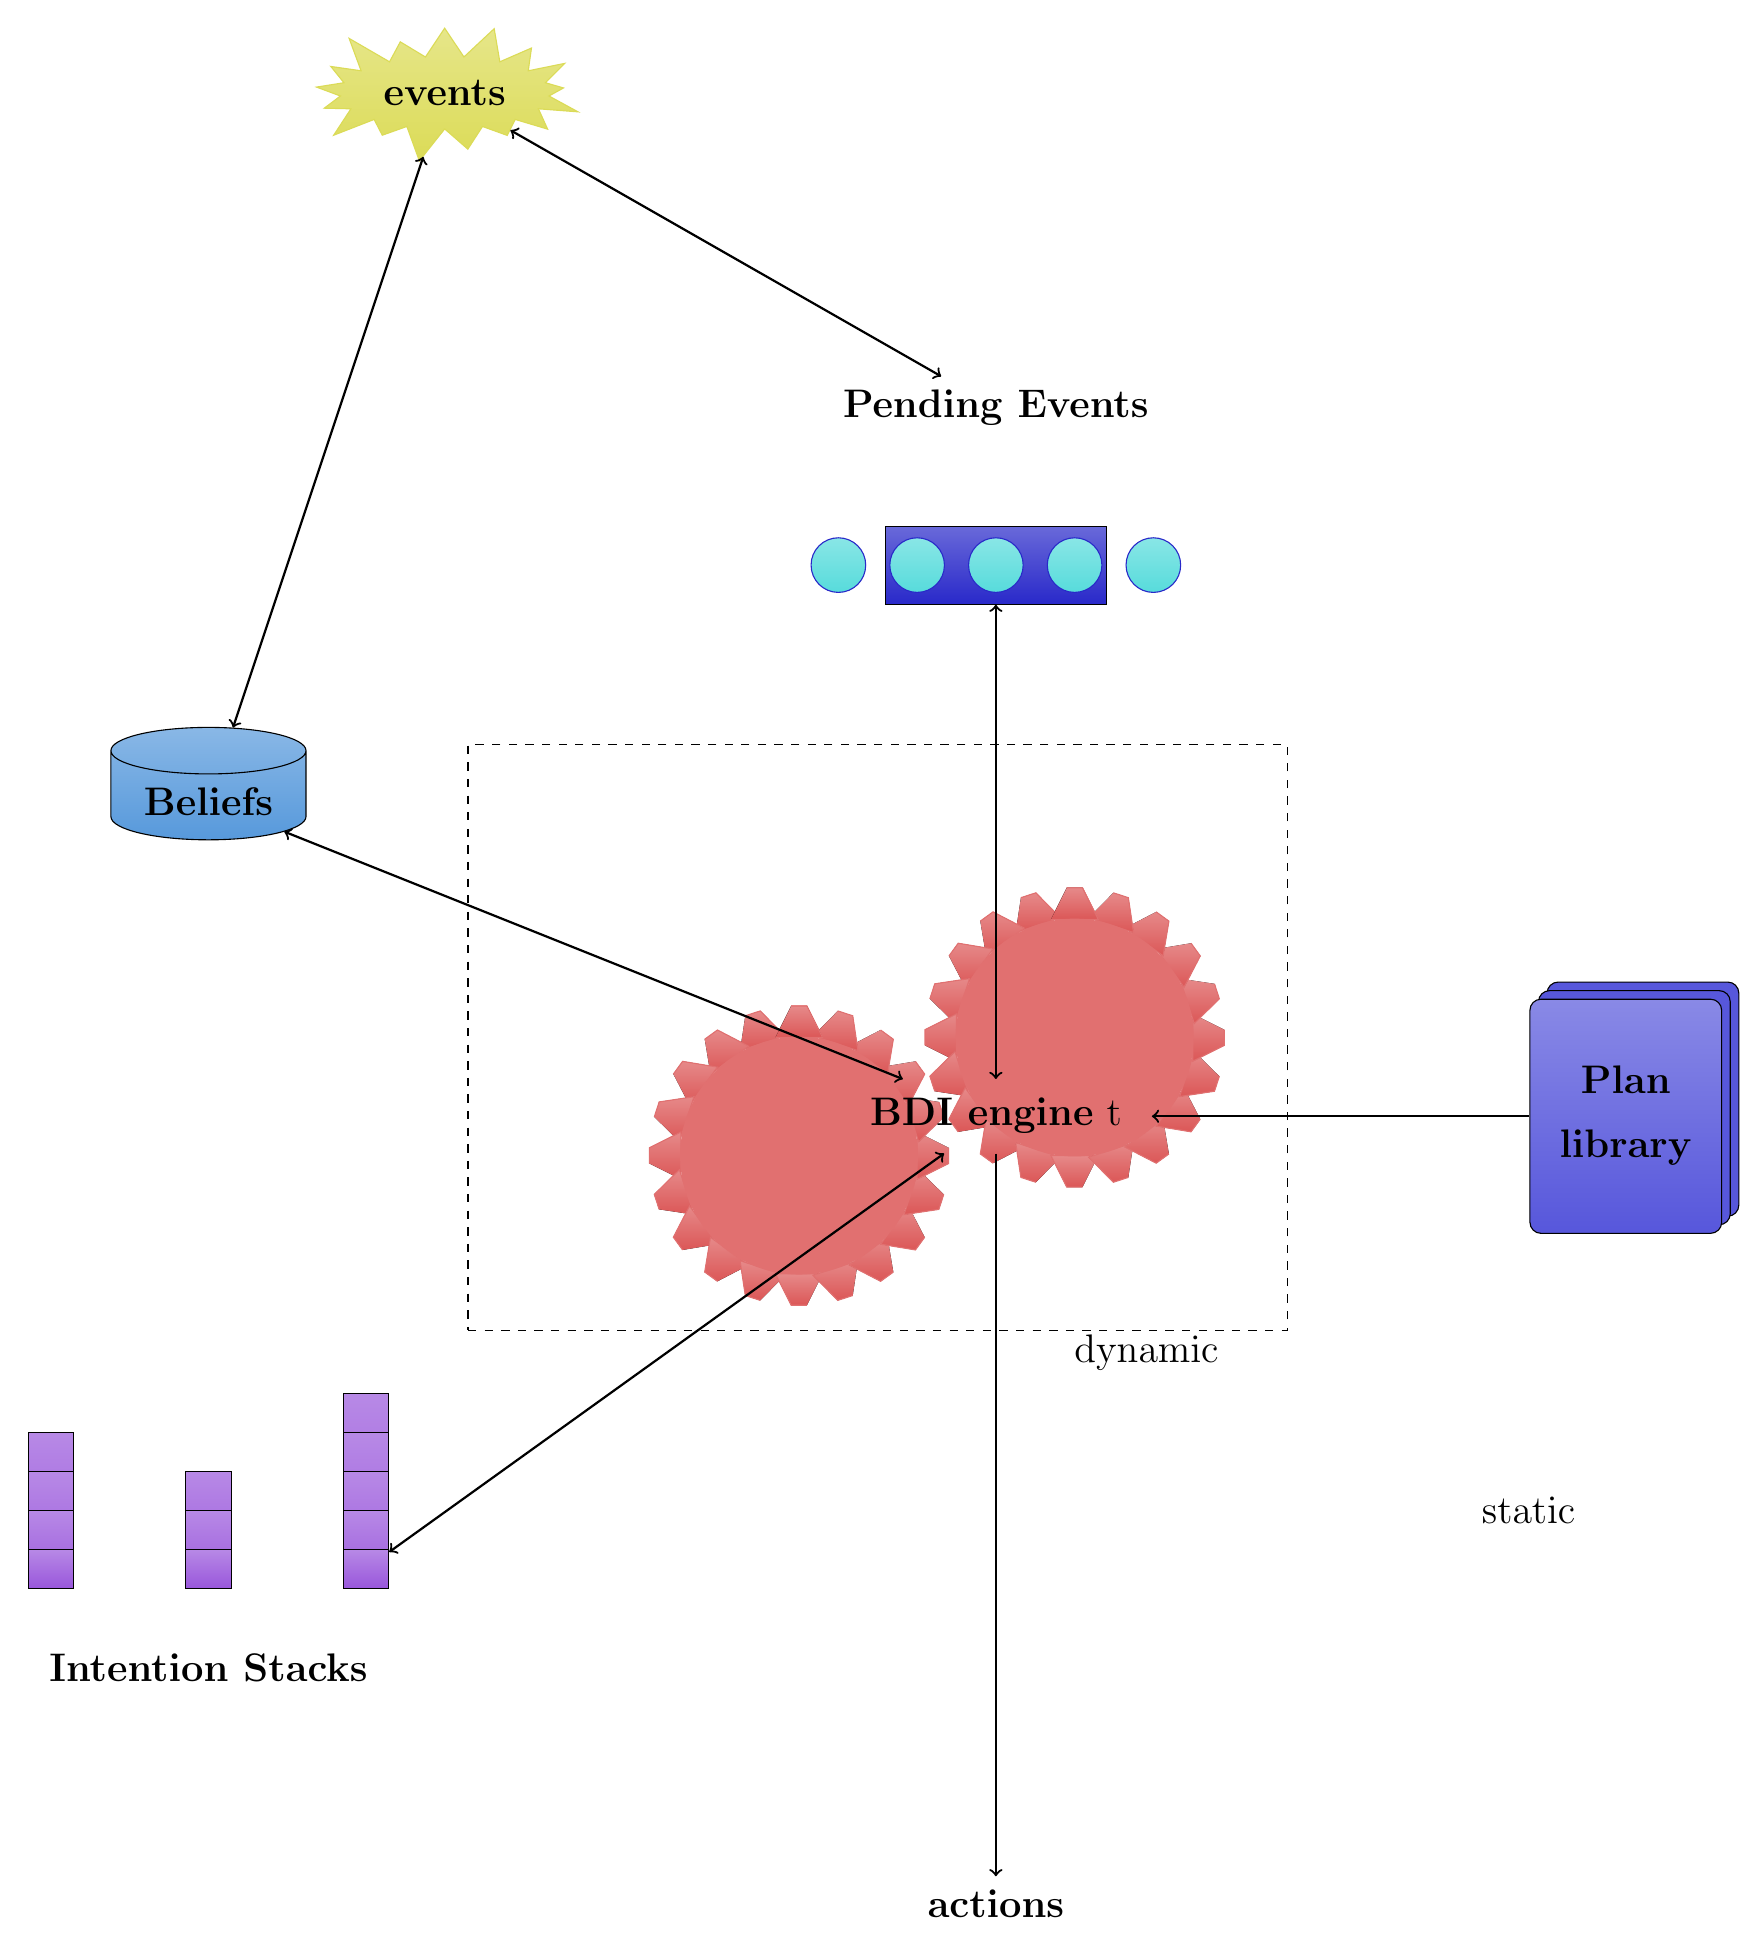
\begin{tikzpicture}

\definecolor{green1}{rgb}{0.86,0.86,0.34}
\definecolor{red1}{rgb}{0.86,0.34,0.34}
\definecolor{blue5}{rgb}{0.6,0.34,0.86}
\definecolor{blue4}{rgb}{0.16,0.16,0.79}
\definecolor{blue3}{rgb}{0.34,0.86,0.86}
\definecolor{blue2}{rgb}{0.34,0.6,0.86}
\definecolor{blue1}{rgb}{0.34,0.34,0.86}

\tikzstyle{centityd}=[draw=black]
\tikzstyle{centityf}=[fill=blue1!30]
\tikzstyle{centity}=[centityd,centityf]
\tikzstyle{entity}=[centity,thick,text centered,anchor=center]



%%% Beliefs
\node (database) at (-3,10)  (B)
	[draw=black,top color=blue2!70, bottom color=blue2,cylinder,shape border rotate=90,minimum width=5em,shape aspect=.3]
	{\textbf{Beliefs}};


%%% Pending Events
\node at (7,15) (eventQueue) {{\bf Pending Events}};
\begin{pgfonlayer}{foreground}
\foreach \x in {5,6,...,9}
\draw [draw=blue4,top color=blue3!70, bottom color=blue3](\x,13) circle (.7em);
\end{pgfonlayer}
\draw (7,13) node (Q) 
	[draw=black,top color=blue4!70, bottom color=blue4,text width=5em, minimum height=2em] {};

%%% Plan Library
\node at (15,6)(P) 
	[draw=black,top color=blue1!70, bottom color=blue1,
	rounded corners, double copy
	shadow={fill=blue1},text centered, 
	minimum height=6em] 
	{	\begin{tabular}{c} 
          \textbf{Plan} \\[1ex]
          \textbf{library}
         \end{tabular}	};
\node[anchor=west] at (13,1) {static};

%%% Intention Stacks
\foreach \x in {4,3,2,1}
\draw (-5,0) node (I) [anchor=south,draw=black,top color=blue5!70, bottom color=blue5,text width=0.5em,
	minimum height=\x em]{};
\foreach \x in {3,2,1}
\draw (-3,0) node (I) [anchor=south,draw=black,top color=blue5!70, bottom color=blue5,text width=0.5em,
	minimum height=\x em]{};
\foreach \x in {5,4,3,2,1}
\draw (-1,0) node (I) [anchor=south,draw=black,top color=blue5!70, bottom color=blue5,text width=0.5em,
	minimum height=\x em]{};
\node at (-3,-1) (Intentions) {{\bf  Intention Stacks}};

%%% BDI Engine
\foreach \x in {0,18,...,360}
\fill [rotate around={\x:(4.5,5.5)}, draw=red1!85, top color=red1!70,bottom color=red1] 
	(4.2,7.0) -- (4.8,7.0) -- (4.6,7.4) -- (4.4,7.4);
\fill [fill=red1!85] (4.5,5.5) circle (1.51);

\foreach \x in {0,18,...,360}
\fill [rotate around={\x:(8.0,7.0)}, draw=red1!85, top color=red1!70,bottom color=red1] 
	(7.7,8.5) -- (8.3,8.5) -- (8.1,8.9) -- (7.9,8.9);
\fill [fill=red1!85] (8.0,7.0) circle (1.51);

\node[anchor=east] at (10,3)  {dynamic};

%%% Events
\node at (0,19) [starburst,draw=green1,top color=green1!70, bottom color=green1] (in) {{\bf events}};

%%% Labels and Arrows
\begin{pgfonlayer}{foreground}
\node[anchor=center] at (7,6)  (deli) 
	{\begin{tabular}{c}
     	\textbf{BDI engine} t
     \end{tabular}};
\node at (7,-4) (actions) {{\bf actions}};
\draw[thick,->] (deli) -- (actions) ; 
\draw[thick,<->] (deli) -- (I) ; 
\draw[thick,<->] (deli) -- (B) ; 
\draw[thick,<-] (deli) -- (P) ;
\draw[thick,<->] (deli) -- (Q) ; 
\draw[thick,<->] (in) -- (eventQueue) ; 
\draw[thick,<->] (in) -- (B) ; 
\end{pgfonlayer}

%%% Encapuslating box
\begin{pgfonlayer}{background}
\node[draw,dashed,rectangle,minimum height=15em,minimum width=21em ] at (5.5,7){};
\end{pgfonlayer}


\end{tikzpicture}}
\vskip 0.5em

A plan is \alert{relevant} for a goal that it was written to handle at design-time. The plan is also \alert{applicable} for that goal if it's context condition are satisfied at run-time. 

\end{textblock}



%%%%% Learning Task
\begin{textblock}{4.6}(5.2,4)
\posterheading{Learning Task}
\vskip 1.0em
\resizebox{\columnwidth}{!}{%!TEX root = ../aamas11storage.tex
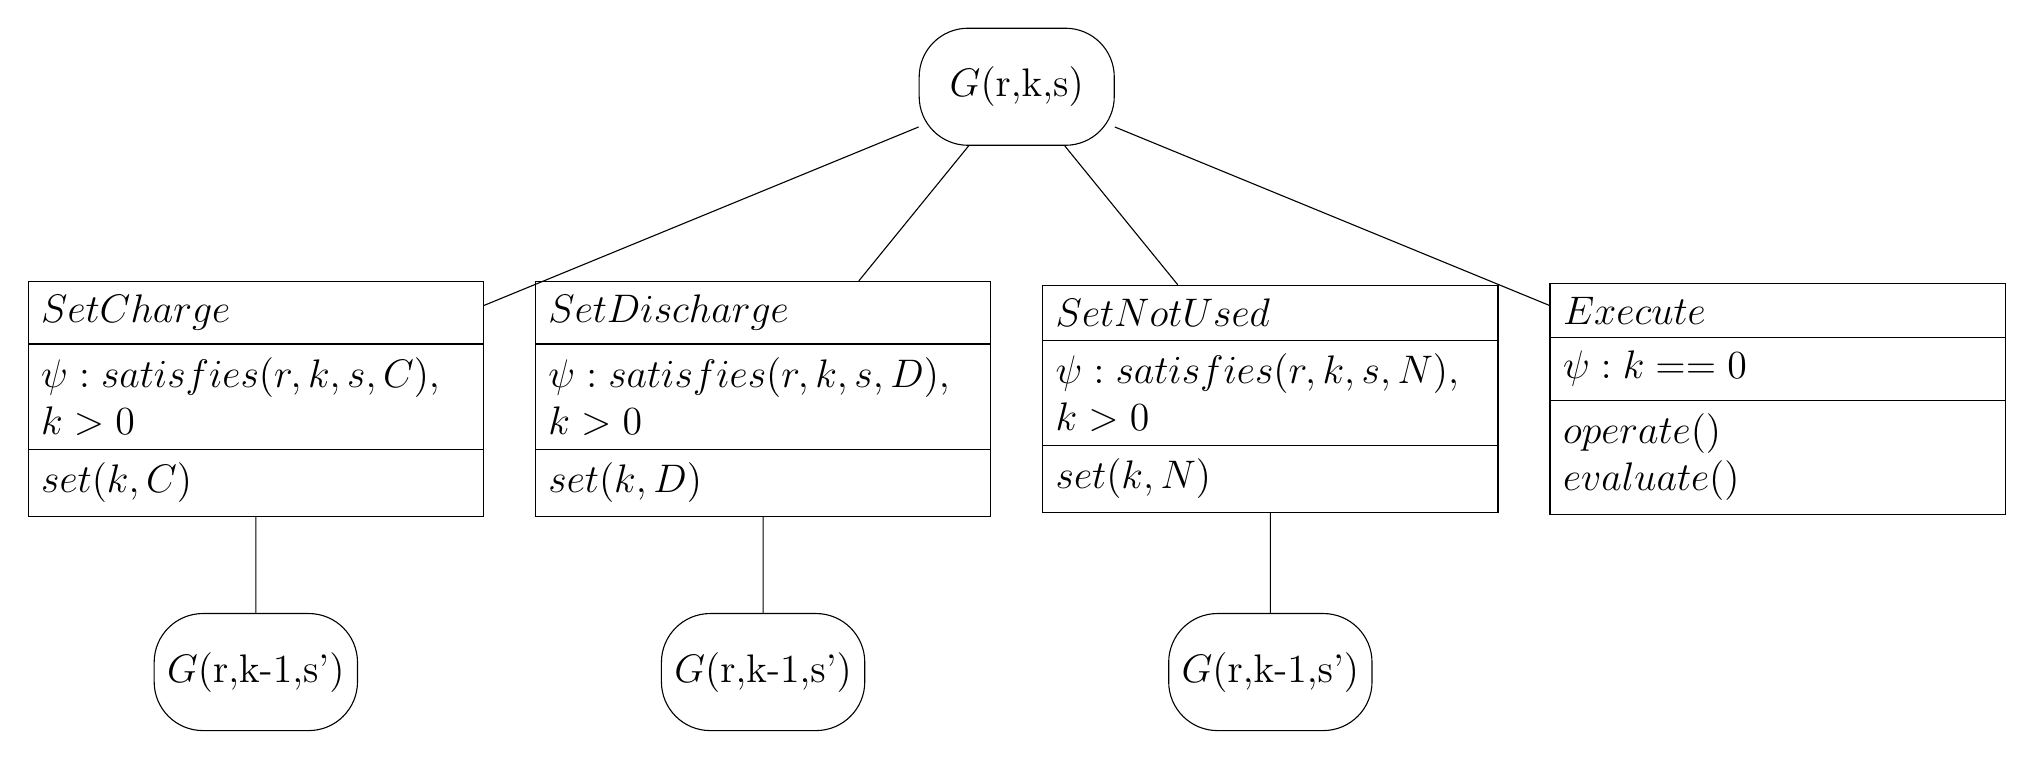
\begin{tikzpicture} [level distance=8.0em]
\tikzstyle{planbox}=[draw,text width=11.0em,rectangle split,rectangle split parts=3]
\tikzstyle{goalbox}=[draw,rounded corners=1.25em,minimum height=3em,minimum width=5em]

	
\tikzstyle{level 1}=[sibling distance=13.0em] 
\tikzstyle{level 2}=[level distance=7.0em] 

\node[goalbox,solid] {$G($r,k,s$)$}
	child {node[planbox] {$SetCharge$ 
			\nodepart{second} $\psi:satisfies(r,k,s,C),$\\$k>0$
			\nodepart{third} $set(k,C)$
		}
		child {node[goalbox] {$G($r,k-1,s'$)$}}
	}
	child {node[planbox] {$SetDischarge$ \nodepart{second}
			\nodepart{second} $\psi:satisfies(r,k,s,D),$\\$k>0$
			\nodepart{third} $set(k,D)$
		}
		child {node[goalbox] {$G($r,k-1,s'$)$}}
	}
	child {node[planbox] {$SetNotUsed$ \nodepart{second}
			\nodepart{second} $\psi:satisfies(r,k,s,N),$\\$k>0$
			\nodepart{third} $set(k,N)$
		}
		child {node[goalbox] {$G($r,k-1,s'$)$}}
	}
	child {node[planbox] {$Execute$ 
			\nodepart{second} $\psi:k==0$
			\nodepart{third} $operate()$ \\$evaluate()$
		}
	}
;

\end{tikzpicture}


}
\vskip 0.5em

First, the imposed BDI hierarchy implies that high level plans may fail not because they were poor choices in the given situation but because poor choices were made further below in the hierarchy. This is the \alert{credit assignment problem} in hierarchical learning.

Second, and regardless of the above, since learning and acting in the environment are interleaved, then care must be taken in how much \alert{confidence} to put in the decision tree on an ongoing basis.
\end{textblock}

%%%%% BDI Learning Framework
\begin{textblock}{4.6}(5.2,15)
\posterheading{BDI Learning Framework}

Each plan's logical formula context condition is augmented with a \alert{decision tree}.

A \alert{probabilistic plan selection function} balances exploitation of ongoing decision tree learning and further exploration of the state space. 

\vskip 2.0em
%\resizebox{\columnwidth}{!}{
\begin{center}
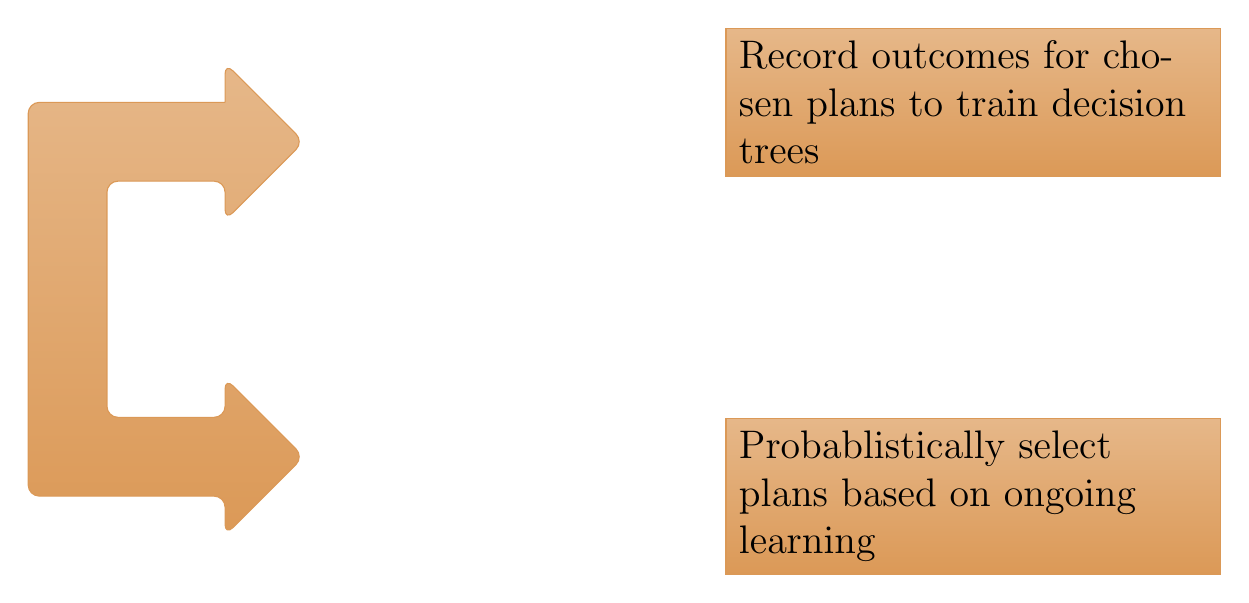
\begin{tikzpicture}
\definecolor{brown3}{rgb}{0.86,0.6,0.34}
	\node [text width=12em, draw=brown3, 
	top color=brown3!70, bottom color=brown3] at (0,0) (A) {
		Record outcomes for chosen plans to train decision trees
	};
	\node [text width=12em, draw=brown3, 
	top color=brown3!70, bottom color=brown3] at (0,-5) (B) {
		Probablistically select plans based on ongoing learning
		};
	\draw [rounded corners,brown3,top color=brown3!70, bottom color=brown3](-9.5,0) -- (-12,0) -- (-12,-5) -- (-9.5,-5) --
	(-9.5,-5.5) -- (-8.5,-4.5) -- (-9.5,-3.5) -- (-9.5,-4.0) --
	(-11,-4) -- (-11,-1) -- (-9.5,-1) -- 
	(-9.5,-1.5) -- (-8.5,-0.5) -- (-9.5,0.5) -- (-9.5,0)
	;
\end{tikzpicture}
\end{center}
%}
\vskip 0.5em
\alert{Acting and learning are interleaved}. Ongoing learning impacts the choice of future actions that impact subsequent learning and whether a good solution is eventually found.

\end{textblock}

%%% Experimentation
\begin{textblock}{4.6}(10.2,4)
\posterheading{Experimentation}

We look at two aspects of learning.

\alert{How to record training set}: We compare two approaches, a conservative BUL scheme that uses only failures where all plan choices were considered well-informed, and the alternative ACL that uses every outcome for learning.

\alert{How to use decision trees}: We present a confidence measure that is applied to the decision tree prediction to calculate final plan selection weights. Confidence is proportional to the \alert{coverage} of paths below a plan.

We experiment with a range of \alert{synthetic hierarchies} to see how each learning approach is impacted by the goal-plan structure.

Sed ut perspiciatis unde omnis iste natus error sit voluptatem accusantium doloremque laudantium, totam rem aperiam, eaque ipsa quae ab illo inventore veritatis et quasi architecto beatae vitae dicta sunt explicabo. Nemo enim ipsam voluptatem quia voluptas sit aspernatur aut odit aut fugit, sed quia consequuntur magni dolores eos qui ratione voluptatem sequi nesciunt. Neque porro quisquam est, qui dolorem ipsum quia dolor sit amet, consectetur, adipisci velit, sed quia non numquam eius modi tempora incidunt ut labore et dolore magnam aliquam quaerat voluptatem. Ut enim ad minima veniam, quis nostrum exercitationem ullam corporis suscipit laboriosam, nisi ut aliquid ex ea commodi consequatur? Quis autem vel eum iure reprehenderit qui in ea voluptate velit esse quam nihil molestiae consequatur, vel illum qui dolorem eum fugiat quo voluptas nulla pariatur?


\end{textblock}


%%%%% Footer
\begin{textblock}{15}(0,24)
\begin{center}
\color{darkred}{\LARGE
D.~Singh, S.~Sardina, L.~Padgham, S.~Airiau, Learning context conditions for
  {BDI} plan selection. In {\it Proceedings of Autonomous Agents and Multi-Agent
  Systems (AAMAS)}, Toronto, Canada, 2010.
}
\end{center}
\end{textblock}

\end{document}